% // ============================================================================
%//
%// Copyright (c) 1999 The CGAL Consortium
%//
%// This software and related documentation is part of an INTERNAL release
%// of the Computational Geometry Algorithms Library (CGAL). It is not
%// intended for general use.
%//
%// ----------------------------------------------------------------------------
%//
%// release       :
%// release_date  :
%//
%// file          : /doc_tex/basic/Triangulation3/Triangulation3.tex
%// revision      : $Revision$
%//
%// author(s)     : Monique Teillaud <Monique.Teillaud@sophia.inria.fr>
%//
%// coordinator   : INRIA Sophia Antipolis (Mariette Yvinec <Mariette.Yvinec@sophia.inria.fr>)
%//
%//============================================================================
\chapter{3D Triangulation}
\label{chapter-Triangulation3}
\begin{ccTexOnly}
\vspace*{-2cm}
\includegraphics{grille.eps} \hspace*{2cm} 
\includegraphics{sphere.eps} 
\end{ccTexOnly}
\begin{ccHtmlOnly}
<img border=0 src="./sphere.gif" align=center>
<img border=0 src="./grille.gif" align=center>
\end{ccHtmlOnly}

The basic 3D-triangulation class of \cgal\ is primarily designed to
represent the triangulations of a set of points $A$ in $\R^3$.  It is
a partition of the convex hull of {$A$} into tetrahedra whose vertices
are the points of {$A$}.  Together with the unbounded cell having the
convex hull boundary as its frontier, the triangulation forms a
partition of $\R^3$. Its cells ($3$-faces) are such that two cells
either do not intersect or share a common facet ($2$-face), edge
($1$-face) or vertex ($0$-face).

\section{Representation}
\label{Triangulation3-sec-intro}

In order to deal
only with tetrahedra, which is convenient for many applications, the
unbounded cell can be subdivided into tetrahedra by considering that
each convex hull facet is incident to an \ccc{infinite cell} having as
fourth vertex an auxiliary vertex called the \ccc{infinite vertex}.  In
that way, each facet is incident to exactly two cells and special cases
at the boundary of the convex hull are simple to deal with.

The class \ccc{Triangulation_3<TriangulationTraits_3,TriangulationDataStructure_3>} of \cgal\ implements this
point of view and therefore considers the triangulation of the set
of points as a set of finite and infinite tetrahedra.  Notice that the
infinite vertex has no significant coordinates and that no
geometric predicate can be applied on it.

A triangulation is a collection of vertices and cells that are linked
together through incidence and adjacency relations. Each cell gives
access to its four incident vertices and to its four adjacent
cells. Each vertex gives access to one of its incident cells.

The four vertices of a cell are indexed with 0, 1, 2 and 3 in positive
orientation, the positive orientation being defined by the orientation
of the underlying Euclidean space $\R^3$. The neighbors of a cell are also
indexed with 0, 1, 2, 3 in such a way that the neighbor indexed by $i$
is opposite to the vertex with the same index. See
Figure~\ref{Triangulation3-fig-orient}.

\begin{figure}[htbp]
\begin{ccTexOnly}
\begin{center} 
\includegraphics{orient.eps} 
\end{center}
\end{ccTexOnly}
\caption{Orientation of a cell (3-dimensional case).
\label{Triangulation3-fig-orient}}
\begin{ccHtmlOnly}
<CENTER>
<img border=0 src="./orient.gif" align=center alt="Orientation of a cell 
(3-dimensional case)">
</CENTER>
\end{ccHtmlOnly}
\end{figure} 

As in the underlying combinatorial triangulation (see
Chapter~\ref{chapter-TDS3}), edges ($1$-faces) and facets ($2$-faces)
are not explicitly 
represented: a facet is given by a cell and an index (the facet
\ccc{i} of a cell \ccc{c} is the facet of \ccc{c} that is opposite to
the vertex with index \ccc{i}) and an edge is given by a cell and two
indices (the edge \ccc{(i,j)} of a cell \ccc{c} is the edge whose
endpoints are the vertices of \ccc{c} with indices \ccc{i} and
\ccc{j}). See Figure~\ref{TDS3-fig-repres}.  

\paragraph{Degenerate Dimensions}
The class \ccc{Triangulation_3<TriangulationTraits_3,TriangulationDataStructure_3>} can also deal with
triangulations whose dimension is less than~3. A triangulation of a
set of points in $\R^d$ covers the whole space $\R^d$ and consists of
cells having $d+1$ vertices: some of them are infinite, they are
obtained by linking the additional infinite vertex to each facet of
the convex hull of the points.
\begin{itemize}
\item {} \emph{dimension 2:} when a triangulation only contains
coplanar points (which is the case when there are only three points), 
it consists of triangular faces.
\item {} \emph{dimension 1:} the triangulation contains only collinear 
points (which is the case when there are only two points), it consists
of edges.
\item {} \emph{dimension 0:} the triangulation contains only one
finite point.
\item {} \emph{dimension -1:} this is a convention to handle the case
when the only vertex of the triangulation is the infinite one.
\end{itemize} 

The same cell class is used in all cases: triangular faces in
2D can be considered as degenerate cells, having only three vertices
(resp. neighbors)
numbered $(0,1,2)$, and one $NULL$ vertex (resp. neighbor);
edges in 1D have only two vertices (resp. neighbors) numbered $0$ and $1$. 

The implicit representation of facets (resp. edges) still holds
for degenerate dimensions (\textit{i.e.}dimensions $<3$) : in
dimension~2, each cell has only one facet of index 3, and 3 edges
$(0,1)$, $(1,2)$ and $(2,0)$; in dimension~1, each cell has one edge
$(0,1)$.  

\paragraph{Validity}
A triangulation of $\R^3$ is said to be \ccc{locally valid} iff

{\bf (a)-(b)} Its underlying combinatorial graph, the triangulation
data structure, is \ccc{locally valid} 
(see Section~\ref{TDS3-sec-intro} of Chapter~\ref{chapter-TDS3})\\
{\bf (c)} Any cell has its vertices ordered according to positive
orientation. See Figure~\ref{Triangulation3-fig-orient}.

When the triangulation is degenerated into a triangulation of
dimension~2, the  geometric validity reduces to:

{\bf (c-2D)} For any two adjacent triangles $(u,v,w_1)$ and $(u,v,w_2)$ with
common edge $(u,v)$, $w_1$ and $w_2$ lie on opposite sides of $(u,v)$
in the plane.

When all the points are collinear, this condition becomes:

{\bf (c-1D)} For any two adjacent edges $(u,v)$ and $(v,w)$, $u$ and
$w$ lie on opposite sides of the common vertex $v$ on the line.

The \ccc{is_valid()} method provided in \ccc{triangulation_3} checks
the local validity of a given triangulation. This does not always
ensure global validity \cite{mnssssu-cgpvg-96,dlpt-ccpps-98} but it is 
sufficient for practical cases.

\section{Software Design}
\label{Triangulation3-sec-design}

The class \ccc{Triangulation_3<TriangulationTraits_3,TriangulationDataStructure_3>} is
designed to be used as  
a layer upon a 3D-triangulation data structure as presented in 
Section~\ref{TDS3-sec-design} of Chapter~\ref{chapter-TDS3}.
It provides high-level geometric operations such as location of a point
in the triangulation and insertion of a point, and is responsible for
the geometric validity. This class is parameterized by two classes:
\begin{itemize}
\item {} the \textbf{geometric traits} class, where the user can
specify the type of points to use as well as the elementary
operations on them (predicates,\ldots). The concept of such a class is
introduced in Section~\ref{Triangulation3-sec-Traits}\lcTex{ and described in 
\ccRefPage{TriangulationTraits_3}} and the homegeneous and cartesian
kernels of \cgal\ are models for this concept
(see also \ccc{CGAL::Regular_triangulation_euclidean_traits_3<R,Weight>}\lcTex{
(\ccRefPage{CGAL::Regular_triangulation_euclidean_traits_3<R,Weight>})} 
for the Regular triangulation).
\item {} the \textbf{triangulation data structure} class of the middle level, 
described in Chapter~\ref{chapter-TDS3}.
\end{itemize}	

Delaunay triangulations as well as triangulation hierarchies
\cite{d-iirdt-98} are also implemented in the package: 
\ccc{Delaunay_triangulation_3<DelaunayTriangulationTraits_3,TriangulationDataStructure_3>}
inherits from  
\ccc{Triangulation_3<DelaunayTriangulationTraits_3,TriangulationDataStructure_3>}, and 
\ccc{Triangulation_hierarchy_3<Tr>} inherits from \ccc{Tr}.

\ccc{Triangulation_3<TriangulationTraits_3,TriangulationDataStructure_3>} derives from
\ccc{Triangulation_utils_3<TriangulationTraits_3,TriangulationDataStructure_3>}, 
which defines a set of tools
working on the indices of vertices in cells\lcTex{ 
(\ccRefPage{CGAL::Triangulation_utils_3})}. 

\subsection{The Geometric Traits}
\label{Triangulation3-sec-Traits}

The first template parameter of the triangulation class
\ccc{Triangulation_3<TriangulationTraits_3,TriangulationDataStructure_3>} of \cgal\ is the geometric traits class.

The geometric traits class must define the geometric
objects (points, segments, triangles and tetrahedra) forming the
triangulation together with a few geometric predicates on these objects:
equality, coordinate comparison, orientation in space, orientation
in case of coplanar points, and collinearity tests.

In addition to the requirements described before, the geometric traits
class of a Delaunay triangulation must define predicates for the
\textit{empty sphere property}.

\cgal\ provides two predefined geometric traits classes
\ccc{Cartesian<R>} and \ccc{Homogeneous<R>} using the kernel
geometric objects and predicates.
These classes are templated with a representation class.
They supply the user with all
the functionalities described for the concepts
\ccc{TriangulationTraits_3}\lcTex{
(\ccRefPage{TriangulationTraits_3})},
\ccc{DelaunayTriangulationTraits_3}\lcTex{
(\ccRefPage{DelaunayTriangulationTraits_3})} and
\ccc{TriangulationHierarchyTraits_3}\lcTex{
(\ccRefPage{TriangulationHierarchyTraits_3})}.
So, any of them can be used as a default traits
class for \ccc{Triangulation_3<TriangulationTraits_3,TriangulationDataStructure_3>},
\ccc{Delaunay_triangulation_3<DelaunayTriangulationTraits_3,TriangulationDataStructure_3>}
and for the parameter \ccc{Tr} of \ccc{TriangulationHierarchy_3<Tr>}.

To be used as the traits class for the regular triangulation provided
by \cgal, a class must provide definitions for the \textit{power tests}.
(See Section~\ref{Triangulation3-sec-class-Regulartriangulation}.)
\ccc{Regular_triangulation_euclidean_traits_3<R,Weight>} is a traits class 
 designed to be used by the class
\ccc{Regular_triangulation_3<RegularTriangulationTraits_3,TriangulationDataStructure_3>}. It provides
\ccc{Weighted_point}, a class for weighted points
provided by the class, which derives from the \cgal\ three dimensional
point class. It supplies
the user with all the functionalities 
described for the concept \ccc{RegularTriangulationTraits_3}\lcTex{
(\ccRefPage{RegularTriangulationTraits_3})}. 
 It can be used as a default traits
class for \ccc{Regular_triangulation_3<RegularTriangulationTraits_3,TriangulationDataStructure_3>}.

\subsection{The Triangulation Data Structure Parameter}
\label{Triangulation3-sec-tds}

The second template parameter of the basic triangulation class
\ccc{Triangulation_3<TriangulationTraits_3,TriangulationDataStructure_3>} is a triangulation 
data structure class.  This class can be seen as a container for the
cells and vertices maintaining incidence and adjacency relations (see
Chapter~\ref{chapter-TDS3}).  A model of this triangulation data
structure is \ccc{Triangulation_data_structure_3}\lcTex{ 
(\ccRefPage{CGAL::Triangulation_data_structure_3<TriangulationVertexBase_3,TriangulationCellBase_3>})}.

A default parameter is defined in all the triangulation classes, so, it 
need not be specified by the user. 

\section{Basic Triangulation}

\ccc{Triangulation_3<TriangulationTraits_3,TriangulationDataStructure_3>} expects a model of a 
\textit{geometric traits class} as its first template argument and a model 
of a \textit{triangulation data structure} as its second argument.

The requirements and defaults for the traits classes are described in
the reference pages for 
\ccc{TriangulationTraits_3}\lcTex{
(\ccRefPage{TriangulationTraits_3})},
\ccc{DelaunayTriangulationTraits_3}\lcTex{
(\ccRefPage{DelaunayTriangulationTraits_3})}, 
\ccc{TriangulationHierarchyTraits_3}\lcTex{
(\ccRefPage{TriangulationHierarchyTraits_3})},
 \ccc{RegularTriangulationTraits_3}\lcTex{
(\ccRefPage{RegularTriangulationTraits_3})}, 
and
\ccc{CGAL::Regular_triangulation_euclidean_traits_3<R,Weight>}\lcTex{
(\ccRefPage{CGAL::Regular_triangulation_euclidean_traits_3<R,Weight>})}.

The requirements and default for the triangulation data structure are
described in Chapter~\ref{chapter-TDS3}. However, a default parameter
is defined in \ccc{Triangulation_3}, so that the user who 
has no additional needs can use
\ccc{Triangulation_3<TriangulationTraits_3>} without specifying the 
second argument.

\section{Delaunay Triangulation} 

The class \ccc{Delaunay_triangulation_3<DelaunayTriangulationTraits_3,TriangulationDataStructure_3>}
represents a three-dimensional Delaunay triangulation. 
This Delaunay triangulation is fully dynamic: it supports both
insertions and vertex removal. 

The user is advised to use the class
\ccc{Triangulation_hierarchy_3<Tr>} in order to benefit from an
increased efficiency. 

\section{Triangulation hierarchy} 

The class \ccc{Triangulation_hierarchy_3<Tr>} implements a
triangulation augmented with a data structure that allows fast point
location queries. Thus, it allows fast construction of the
triangulation. As proved in~\cite{d-iirdt-98}, this structure has an
optimal behaviour when it is built for Delaunay triangulations.
However it can be used as well for other triangulations and the
\ccRefName\ class is templated by a parameter, which is to be
instantiated by one of the \cgal\ triangulation classes.  It offers
the same functionalities as the \ccc{Tr} parameter class. 

Note that, since the algorithms that are provided are randomized, the
running time of constructing a triangulation with a hierarchy may be
improved when shuffling the data points.

\section{Regular Triangulation} 
\label{Triangulation3-sec-class-Regulartriangulation}

\ccc{Regular_triangulation_3<RegularTriangulationTraits_3,TriangulationDataStructure_3>}
implements incremental regular triangulations.

Let ${S}^{(w)}$ be a set of weighted points in $\R^3$. Let
${p}^{(w)}=(p,w_p), p\in\R^3, w_p\in\R$ and 
${z}^{(w)}=(z,w_z), z\in\R^3, w_z\in\R$ be two weighted points. 
A weighted point
${p}^{(w)}=(p,w_p)$ can also be seen as a sphere of center $p$ and
radius $w_p$. 
The \textit{power product} between ${p}^{(w)}$ and ${z}^{(w)}$ is
defined as 
\[\Pi({p}^{(w)},{z}^{(w)}) = {\|{p-z}\|^2-w_p^2-w_z^2}\]
where $\|{p-z}\|$ is the Euclidean distance between $p$ and $z$. 
 ${p}^{(w)}$ and ${z}^{(w)}$
are said to be \textit{orthogonal} if $\Pi{({p}^{(w)}-{z}^{(w)})}
= 0$ (see Figure~\ref{Triangulation3-fig-ortho}).

\begin{figure}[htbp]
\begin{ccTexOnly}
\begin{center} 
\includegraphics{ortho.eps} 
\end{center}
\end{ccTexOnly}
\caption{Orthogonal weighted points (picture in 2D).
\label{Triangulation3-fig-ortho}}
\begin{ccHtmlOnly}
<CENTER>
<img border=0 src="./ortho.gif" align=center alt="Orthogonal weighted
points (picture in 2D)"> 
</CENTER>
\end{ccHtmlOnly}
\end{figure} 

Four weighted points have a unique common orthogonal weighted point
called the \textit{power sphere}.  The weighted point orthogonal to
three weighted points in the plane defined by these three points is
called the \textit{power circle}. The
\textit{power segment} will denote the weighted point orthogonal to
two weighted points on the line defined by these two points.

A sphere ${z}^{(w)}$ is said to be
\textit{regular} if $\forall {p}^{(w)}\in{S}^{(w)},
\Pi{({p}^{(w)}-{z}^{(w)})}\geq 0$.

A triangulation of ${S}^{(w)}$ is \textit{regular} if the power spheres
of all simplices are regular. 

The regular triangulation of
${S}^{(w)}$ is in fact the projection onto $\R^3$ of the convex hull 
of the four-dimensional points $(p,\|p-O\|^2-w_p),$ for
${p}^{(w)}=(p,w_p)\in{S}^{(w)}$. 
Note that all points of ${S}^{(w)}$ do not
necessarily appear as vertices of the regular
triangulation. To know more about regular triangulations, see for
example \cite{es-itfwr-96}. 

When all weights are 0, power spheres are nothing more than
circumscribing spheres, and the regular triangulation is exactly the
Delaunay triangulation.

%\section{Debugging}

%	\subsection{Pretty print}	
% \textit{to be written}

%	\subsection{Debugging with handles} 
%Most debuggers cannot understand \ccc{handles} well. Under the
%debugger, an instruction such as

%\texttt{(dbx) print -r c->vertex(0)}

%where \ccc{c} is a \ccc{Cell_handle}, is answered by:

%\texttt{can't find field "vertex" in "c"}

%To work around this problem, two functions have been defined to transform 
%\ccc{handles} into usual $C^{++}$ pointers for debugging purposes.

%\ccFunction{template <class Triangulation_traits_3, class Tds_3>
%	Triangulation_vertex_3<Triangulation_traits_3,Tds_3> * 
%debug(const Triangulation_vertex_handle_3<Triangulation_traits_3,Tds_3> v);}
%{}

%\ccFunction{template <class Triangulation_traits_3, class Tds_3>
%	Triangulation_cell_3<Triangulation_traits_3,Tds_3> * 
%	debug(const Triangulation_cell_handle_3<Triangulation_traits_3,Tds_3>
%c);}
%{}

%This allows the following:\\
%\texttt{(dbx) print -r CGAL\_debug(c)->vertex(0)\\
%CGAL\_debug(c)->vertex(0) = \{\\\
%\ldots\\
%\} }



\section{Examples}
\label{Triangulation3-sec-examples}
\subsection{First example}
This example shows the incremental construction of a 3D triangulation, 
the location of a point, and how to manipulate elementary operations
on indices in a cell. It uses the default parameters proposed by
\cgal\ for the \ccc{Triangulation_3} class.

\ccIncludeExampleCode{Triangulation_3/example_simple.C}

\subsection{Example changing the vertex base}
This example shows how the user can plug his own vertex base in a
triangulation.

\ccIncludeExampleCode{Triangulation_3/example_color.C}

\subsection{Use of the Delaunay Hierarchy}

\ccIncludeExampleCode{Triangulation_3/example_hierarchy.C}
